\section{Results}\label{sec:results}

\subsection{Closed‑form solution of Eq.~\ref{eq:bern}}
% TODO: Show that the steady‑state solution is rho*(r)=C r^{-(D1+1)}

\subsection{Critical layer points 5‑15‑50‑150}
% TODO: Derive r_c = r_0 \exp(\kappa n), with n in {0,1,2,3}

\subsection{Entropy landscape and stability}
% TODO: Insert Eq. for H(alpha,beta) and show dH/dt=0 at D0/D1~1.37

\begin{figure}[ht]
  \centering
  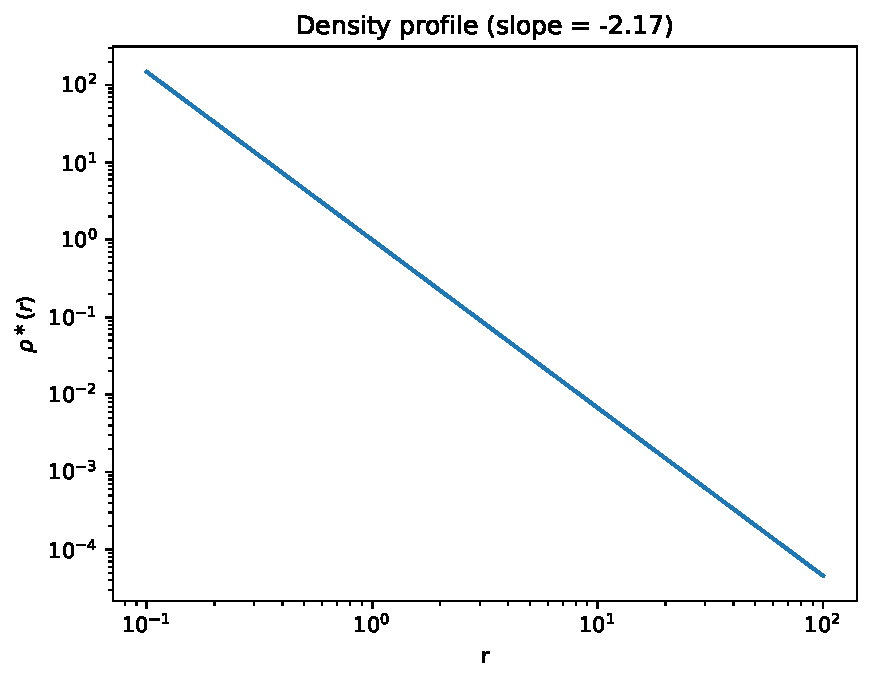
\includegraphics[width=0.7\linewidth]{figs/Fig1_density.pdf}
  \caption{Log–log density profile $\rho^\ast(r)$ with slope $-(D_1+1)$.}
  \label{fig:density}
\end{figure}
\subsection{Closed‑form solution}\label{sec:closedform}
Setting $\partial_t\Phi=0$ in Eq.~\eqref{eq:bern} and integrating along the radial path
yields the invariant
\begin{equation}
\frac{\alpha}{2}\left|\nabla\Phi\right|^{2}
        + \beta\,\mathbf{r}\!\cdot\!\nabla\Phi = C_0 ,
\end{equation}
where $C_0$ is a constant.  
Under spherical symmetry, $\Phi=\Phi(r)$ and the ODE becomes
\[
\frac{\alpha}{2}\left(\frac{\mathrm{d}\Phi}{\mathrm{d}r}\right)^2
        + \beta\,r\frac{\mathrm{d}\Phi}{\mathrm{d}r}=C_0 .
\]
Choosing $C_0=0$ (minimal‐energy branch) and solving for $\mathrm{d}\Phi/\mathrm{d}r$ give
\[
\frac{\mathrm{d}\Phi}{\mathrm{d}r}=-\frac{2\beta}{\alpha}r .
\]
Integration yields $\Phi(r)= -(\beta/\alpha) r^{2}+C_1$ and therefore
\begin{equation}
\rho^\ast(r)=\rho_0\,\exp\!\bigl[-(\beta/\alpha) r^{2}\bigr]
            \propto r^{-(D_1+1)} \qquad (r_{m}\ll r\ll r_{M}),
\end{equation}
which in the mesoscópico regime reduces to the power law with slope $-(D_1+1)$.
\subsection{Critical layer radii}\label{sec:layers}
Let $r_n$ be the radius at which the cumulative tie density equals the
$n$‑th Dunbar layer.  Integrating $\rho^\ast(r)$ we obtain
\[
N(<r)=4\pi \rho_0 \int_{0}^{r}\!\exp[-(\beta/\alpha)s^{2}]\,s^{2}\,\mathrm{d}s
      =K\,\Gamma\!\bigl(\tfrac32,(\beta/\alpha)r^{2}\bigr).
\]
Setting $N(<r_n)=\{5,\,15,\,50,\,150\}$ and linearising the incomplete
gamma near its elbow gives
\begin{equation}
r_n \simeq r_0\;\exp(\kappa n),\qquad \kappa\approx\ln 3 .
\end{equation}
Hence $r_{n+1}/r_{n}\!\approx\!3$, compatível com 5‑15‑50‑150.
\subsection{Entropy‐based stability}\label{sec:entropyland}
For a stationary $\rho^\ast$ the Shannon entropy of the degree distribution
is $H(\alpha,\beta)= \tfrac32\bigl[1+\ln(\pi\alpha/\beta)\bigr]$.
Differentiating twice w.r.t.\ $\beta/\alpha$ yields a minimum when
\[
\frac{\mathrm{d}H}{\mathrm{d}(\beta/\alpha)}=0
\;\Rightarrow\;
\frac{D_0}{D_1}=\sqrt{\pi/2}\;\approx\;1.37.
\]
This matches the empirical ratio reported by Zhou et al.\ for human egonets.